%% TITLE	Physiological Fluid Mechanics, Summary 5

%% AUTHOR	BINGHUAN W LI (Dept. Chemical Eng/Bio Eng, Imperial)
%%          PETER Y XIE (Dept. Mech Eng, Stanford)

%% compiled in XeLaTeX with Tex Live version 2023.

%% This work is licensed under a Creative Commons Attribution-NonCommercial 4.0 International License.

%=========================================================
%% Reference
%% - dimensional analysis https://projects.exeter.ac.uk/fluidflow/Courses/FluidDynamics3211-2/DimensionalAnalysis/dimensionalLecturese4.html
%=========================================================
%=====================================================
% 11 Sep 2024
% 1. fix errors in dim analy example
% 2. add table 2
% 3. trim table 1, remove items that may be not used in this course
% 4. rephrased derivation of stokes flow equations
% 5. add fig 1 and fig 2, removed the old figure
%=====================================================

\documentclass[a4paper]{article}
\def\NotesType{1}
\def\summaryNo{5}
\def\finalise{1}
%% TITLE	Physiological Fluid Mechanics, configuration

%% DATE		- Nov 19, 2023     create

%% AUTHOR	BINGHUAN W LI (Dept. Chemical Eng/Bio Eng, Imperial)
%%          PETER Y XIE (Dept. Mech Eng, Stanford)

%% compiled in XeLaTeX with Tex Live version 2023.

%% This work is licensed under a Creative Commons Attribution-NonCommercial 4.0 International License.

\usepackage[sfdefault]{arimo}
\usepackage[left=1.5cm, right=1.5cm, top=2cm, bottom=1.5cm]{geometry}
\usepackage{amsmath, amsfonts, amssymb, cancel}
\usepackage{unicode-math}
\setmathfont
    [    Extension = .otf,
         BoldFont = XITSMath-Bold,
    ]{XITSMath-Regular}

% % \DeclareMathSizes{10}{12}{10}{9}

% \usepackage{siunitx}
\usepackage{enumitem}
\usepackage{xcolor}
    \definecolor{linkcolour}{rgb}{0,0.2,0.6}
\usepackage{hyperref}
\hypersetup{
    colorlinks,
    breaklinks,
    urlcolor=linkcolour,
    linkcolor=linkcolour,
    citecolor=black,
    pdfauthor={Li, Binghuan W},
    }
\usepackage{graphicx, float}
\usepackage{framed}
\usepackage[export]{adjustbox}

\usepackage{fancyhdr}
    \pagestyle{fancy}
    \fancyhf{}
    \lhead{\textsc{Physiological Fluid Mechanics Summary \summaryNo}}
    \rhead{page \thepage}

\usepackage{tcolorbox}

\usepackage{tikz, circuitikz}

\usepackage{multicol}
    \setlength{\columnseprule}{1pt}

\usepackage{lscape}

\usepackage{booktabs}

\usepackage{pifont}

\setlength\parindent{0pt}

\newcommand{\Aa}[0]{\boldsymbol{\color{red}a}}
\newcommand{\bb}[0]{\boldsymbol{\color{blue}b}}
\newcommand{\cc}[0]{\boldsymbol{\color{orange}c}}
\newcommand{\dd}[0]{\boldsymbol{\color{purple}d}}

\begin{document}

\section{Dimensional Analysis}
\paragraph{Buckingham-$\Pi$ Theorem} The Buckingham-$\Pi$ theorem states that if an equation involving $k$ variables is dimensionally homogeneous (\textit{i.e.}, L.H.S. units = R.H.S. units), 
\[
    u_1 = f(u_2, u_3, ..., u_k),
\]
it can be reduced to a relationship among $(k-r)$ independent dimensionless products, where $r$ is the minimum number of reference dimensions required to describe the variables,
\[
    \Pi_1 = \phi(\Pi_2, \Pi_3, ... \Pi_{k-r}).
\]

% \begin{tcolorbox}[title = \textbf{Example}, breakable]
% \paragraph{Objective} Perform the dimensional analysis of the scenario where the pressure drops per unit length along a smooth pipe.  \\

% \begin{enumerate}[label=\underline{\textbf{Step \arabic*}}]
%     \item List all relevant variables in the objective equation to be non-dimensionalised. Here, 
%     \[
%     \Delta p_l = f (D, \rho, \mu, V),
%     \]
%     where the pressure drop $\Delta p_l$ is a function of the pipe diameter $D$, the density $\rho$, the (dynamic) viscosity $\mu$, and velocity $V$.

%     \item List the dimensions of the variables. Let [$M$] denotes the dimension of mass, [$L$] denotes the dimension of length, [$T$] denotes the dimension of time, {\color{gray}(refer to \autoref{tab:dim_less_common_params})}
%     \begin{center}
%     \begin{tabular}{lcl}
%          $\Delta p_l \doteq [M L^{-1} T^{-2}]$, && 
%          $\mu \doteq [M L^{-1} T^{-1}]$  \\
%          $D \doteq [L]$,  &&  $V \doteq [L T^{-1}]$\\
%          $\rho \doteq [M L^{-3}] $
%     \end{tabular}
%     \end{center}
    
%     There are $k = 5$ variables and $r = 3$ reference dimensions, we conclude there will be $k-r = 2$ dimensionless groups.

%     \item Suppose the first group involves $\Delta p_l$, $\rho$, $V$ and $D$. Let $\Aa$, $\bb$, $\cc$, $\dd$ denote 4 constants to be determined,
%     \[
%         D^{\Aa} \rho^{\bb} V^{\cc} \Delta p_l^{\dd} 
%         \quad \Longrightarrow \quad 
%         \boxed{[L]^{\Aa}
%         [M L^{-3}]^{\bb} 
%         [LT^{-1}]^{\cc} 
%         [M L^{-1} T^{-2}]^{\dd} 
%         \doteq [L]^0 [F]^0 [T]^0}.
%     \]
%     Balance of $[M]$, $[L]$, $[T]$ would give the simultaneous equations
%     \begin{align*}
%         \text{(mass)} \quad \quad & \bb + \dd = 0, \\
%         \text{(length)} \quad \quad & \Aa - 3\bb + \cc - \dd = 0 ,\\
%         \text{(time)} \quad \quad & -\cc - 2\dd = 0.
%     \end{align*}
%     {\color{gray}(3 equations with 4 unknowns $\Rightarrow$ the equation system is underdetermined, we will not be able to explicitly solve the numerical values of 4 parameters, but at least we will know the relations between $a$, $b$, $c$, $d$.)}\\
    
%     resulting in the following relations: $\Aa = 0$, $\bb = -\dd$, $\cc = -2\dd$. Hence, with $\dd = -1$, $\longrightarrow \Aa = 0$, $\bb = 1$, $\cc = 2$,
%     \[
%         D^0 \rho^1 V^{2} \Delta p_l^{-1} \equiv \left(\frac{\rho V^2}{\Delta p_l} \right) \quad \text{is dimensionless}, \quad \Longrightarrow \quad \boxed{\Pi_1 = \left(\frac{\rho V^2}{\Delta p_l} \right)}.
%     \]
%     {\color{gray}(Although we \textit{supposed} that $D$ might get involved in the first $\Pi$ group, but by $a=0$, $\Pi_1$ is invariant of $D$.)}\\

%     \item Similarly, the second term involves $\mu$, follow the same rule, this yields $\displaystyle \boxed{\Pi_2 = \frac{\mu}{\rho DV}}$, which is $1/{\rm Re}$.

%     \item Hence, we can express the result of the dimensional analysis as
%     \[
%         \frac{\rho V^2}{\Delta p_l} = \phi \left( \frac{\mu}{\rho DV} \right).
%     \]
% \end{enumerate}
% \end{tcolorbox}

\begin{table}[H]
    \centering
    \begin{tabularx}{.9\textwidth}{>{\centering\arraybackslash}m{.15\textwidth} >{\centering\arraybackslash}m{.2\textwidth} >{\centering\arraybackslash}m{.15\textwidth} >{\centering\arraybackslash}m{.3\textwidth}}
    \toprule
        \multicolumn{4}{l}{\textbf{Variables}: Acceleration of gravity, $g$; Bulk modulus, $E_v$; Characteristic length, $L$; Density, $\rho$;}\\
        \multicolumn{4}{l}{Frequency of oscillating flow, $\omega$; Pressure, $p$; Speed of sound, $c$; Surface tension, $\sigma_s$ ; Velocity, $U$.}\\
    \toprule
        \textbf{Dimensionless group}    &   \textbf{Name}    &   \textbf{Interpretation}   &   \textbf{Types of Applications}\\
    \toprule
        $\rho U L/\mu$    &   Reynolds number, $\rm Re$   &   $\frac{\text{inertia force}}{\text{viscous force}}$  & Generally of importance in all types of fluid dynamics problems\\
    \midrule
        $U/\sqrt{gL}$    &   Froude number, $\rm Fr$   &   $\frac{\text{inertia force}}{\text{gravitational force}}$   &   Flow with a free surface\\
    \midrule
        $p/\rho U$    &   Euler number, $\rm Eu$   &   $\frac{\text{pressure force}}{\text{inertia force}}$   &   Problems in which pressure, or pressure differences, are of interest\\
    \midrule
        $U/c$    &   Mach number, $\rm Ma$   &   $\frac{\text{inertia force}}{\text{compressibility force}}$  &   Flows in which the compressibility of the fluid is important\\
    \midrule
        $\omega L/U$    &   Strouhal number, $\rm St$   &   $\frac{\text{inertia(local) force}}{\text{inertia (convective) force}}$    &   Unsteady flow with a characteristic frequency of oscillation\\
    \midrule
        $\rho U^2 L/\sigma_s$    &   Weber number, $\rm We$   &   $\frac{\text{inertia force}}{\text{surface tension force}}$    &   Problems in which surface tension is important\\
    \bottomrule
    \end{tabularx}
    \caption{Common variables and dimensionless groups in fluid mechanics.}
\end{table}

\begin{table}[h]
    \centering
    \begin{tabular}{lll|lll}
        \toprule
        \textbf{Parameter} & \textbf{Symbol} & \textbf{Dimensions} & \textbf{Parameter} & \textbf{Symbol} & \textbf{Dimensions} \\
        \midrule
        Acceleration           & \( a \)             & \( [L^1 T^{-2}] \)   & Surface tension        & \( \sigma_s \)      & \( [M^1 T^{-2}] \)   \\
        Angle                  & \( \theta, \phi, \text{etc.} \) & 1 (none)   & Velocity               & \( U \)             & \( [L^1 T^{-1}] \)   \\
        Density                & \( \rho \)         & \( [M^1 L^{-3}] \)   & Viscosity              & \( \mu \)           & \( [M^1 L^{-1} T^{-1}] \)   \\
        Force                  & \( F \)             & \( [M^1 L^1 T^{-2}] \)   & Volume flow rate       & \( Q \)       & \( [L^3 T^{-1}] \)   \\
        Frequency              & \( f \)             & \( [T^{-1}] \)   & Pressure               & \( p \)             & \( [M^1 L^{-1} T^{-2}] \)   \\
        \bottomrule
    \end{tabular}
    \caption{Table of parameters with symbols and primary dimensions in two columns. $[M]$: mass, $[T]$: time; $[L]$: length.}
    \label{tab:dim_less_common_params}
\end{table}


\section{Non-Dimensional Navier-Stokes Equation}
\begin{itemize}
    \item Define the non-dimensional variables
    \[
        \mathbf{x}^* = \frac{\mathbf{x}}{L},
        \quad \quad
        \mathbf{u}^* = \frac{\mathbf{u}}{U},
        \quad \quad
        t^* = \frac{t}{L/U},
        \quad \quad
        p^* = \frac{p}{P_0},
    \]
    where $L$, $U$ are the characteristic length and velocity, respectively.
    
    \item The dimensionless Navier-Stokes momentum equation is
     \[ 
        {\rm Re}\bigg(\frac{\partial \mathbf{u^{*}}}{\partial t^{*}} + (\mathbf{u^{*}}\cdot \nabla^{*})\mathbf{u^{*}} \bigg) = -\frac{P_{0}}{\frac{\mu U}{L}}\nabla^{*} p^{*} + \nabla^{*2}\mathbf{u^{*}},
     \]
    where $\displaystyle P_{0} = \frac{\mu U}{L}\max(1,{\rm Re})$, \textit{i.e.}, the viscous scale ($\rm Re < 1$) or dynamic scale  ($\rm Re > 1$). This formulation ensures the pressure term has the same order of magnitude as other terms, since there is no natural scaling for pressure.

    \item The dimensionless continuity equation is
     \[ \nabla^{*} \cdot \mathbf{u}^{*} = 0.\]
\end{itemize}

\paragraph{Small $\rm Re$ flow ($ \rm Re \ll 1$)} $P_0 = \mu U/L$ and the L.H.S. eliminated,
\[ 
    \cancelto{0}{{\rm Re}\bigg(\frac{\partial \mathbf{u^{*}}}{\partial t^{*}} + (\mathbf{u^{*}}\cdot \nabla^{*})\mathbf{u^{*}} \bigg)} = -\nabla^{*} p^{*} + \nabla^{*2}\mathbf{u^{*}}
    \quad \Longrightarrow \quad
    \nabla^{*} p^{*} = \nabla^{*2}\mathbf{u^{*}}
    \quad \Longleftrightarrow \quad
    \mu \nabla^2 \mathbf{u} = \nabla p
\]
which is known as the \textbf{Stokes equation} that can be solved analytically due to its linearity. 
\begin{tcolorbox}[breakable, title={\textbf{Governing Equation of Stokes Flow}}]
Define the vorticity as $\boldsymbol{\omega} = \nabla \times \mathbf{u}$
    \[
        \mu \nabla^2 \mathbf{u} = - \mu \nabla \times \boldsymbol{\omega}
        \quad \quad \text{due \ to} \quad \quad
        \nabla \times \boldsymbol{\omega} = \nabla \times (\nabla \times \mathbf{u}) = \cancel{\nabla \cdot \mathbf{u}} - \nabla^2 \mathbf{u}.        
    \]
Further, take the curl of $\mu \nabla^2 \mathbf{u} = \nabla p$:
    \begin{align*}
         \underbrace{\nabla \times \nabla p}_{\substack{\text{``curl of grad} \\ \text{is zero''}}} = \nabla \times (\mu \nabla^2 \mathbf{u})
         \quad \Longrightarrow \quad 
         & 0 \ = \ -\mu \nabla \times (\nabla \times \boldsymbol{\omega}) \\[-2em]
         & 0 \ = \ -\mu [ \underbrace{\nabla (\nabla \cdot \boldsymbol{\omega}) - \nabla^2 \boldsymbol{\omega}}_{\text{by} \ \nabla \times \left( \nabla \times \textbf{A} \right) = \nabla \left( \nabla \cdot \textbf{A} \right) -\nabla^2 \textbf{A}}] \\
         & 0 \ = \ -\mu [\underbrace{\nabla (\nabla \cdot \nabla \times \mathbf{u})}_{\substack{\text{``div of curl} \\ \text{is zero''}}} - \nabla^2 \boldsymbol{\omega}] .
    \end{align*}

The above derivation results in $\nabla^2 \boldsymbol{\omega} = 0$, which is the governing equation of the Stokes flow.
\end{tcolorbox}


\begin{figure}[H]
    \centering
    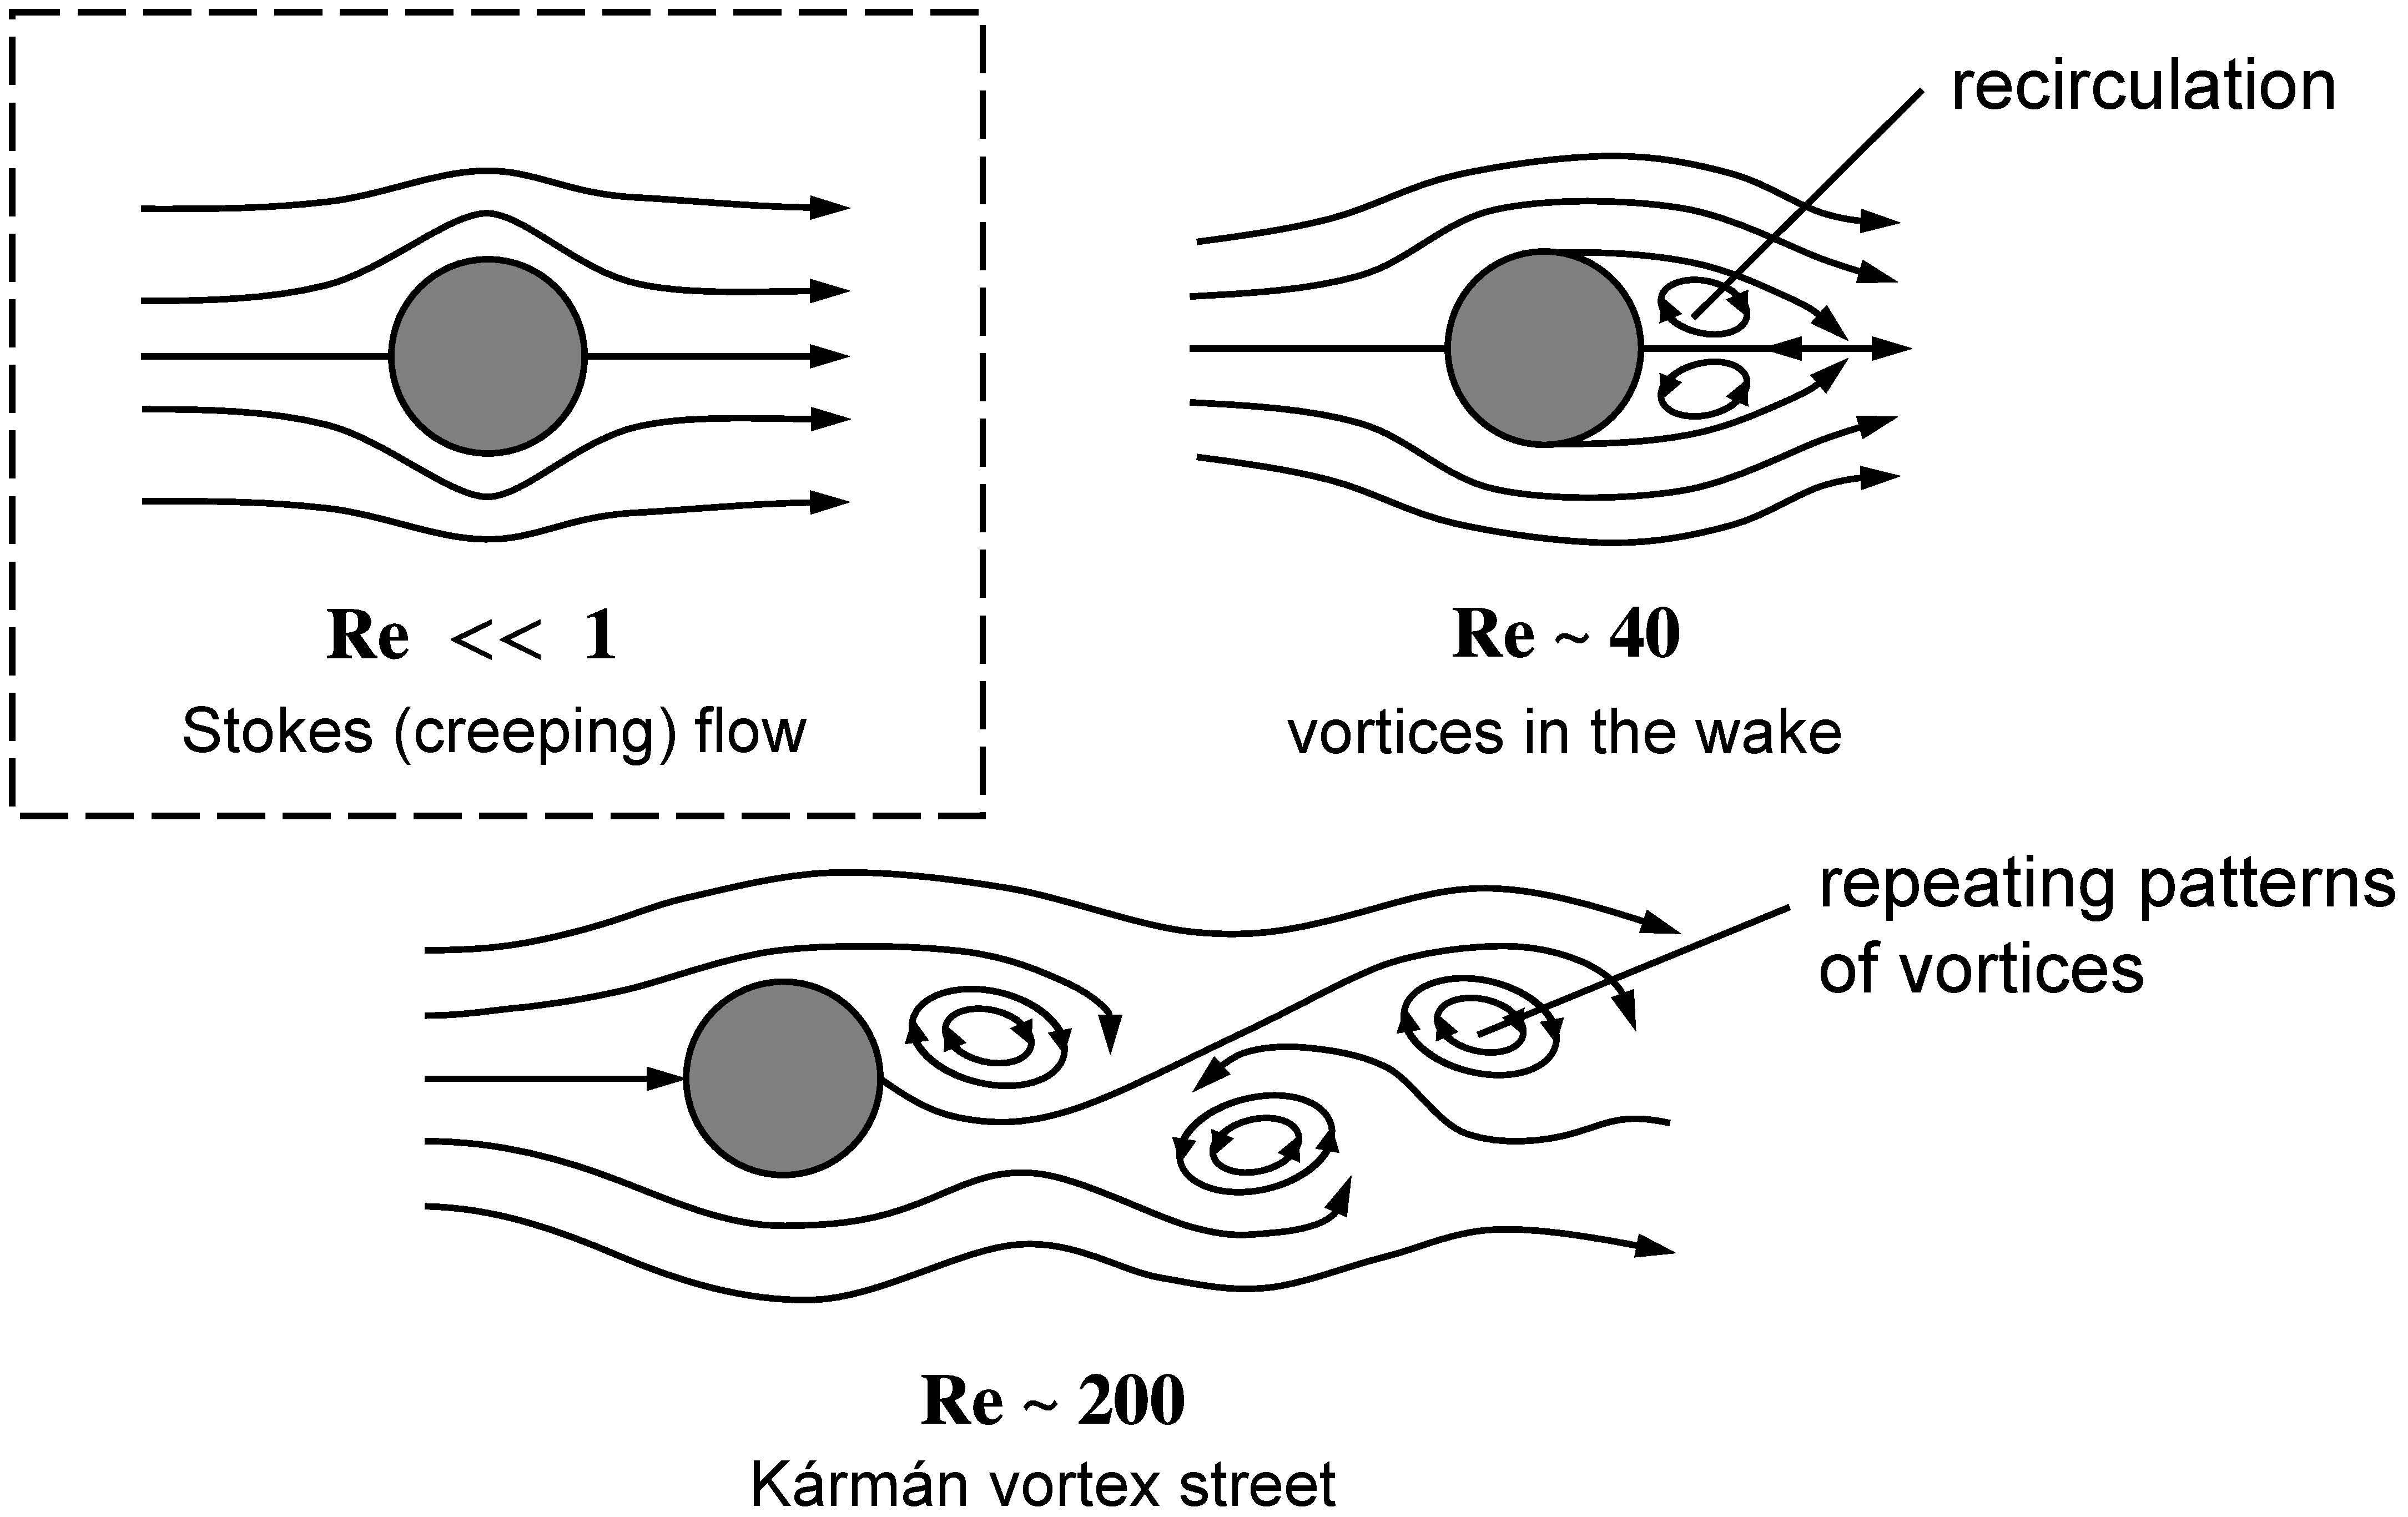
\includegraphics[width=0.6\linewidth]{img/flow_pass_cylinder.eps}
    \caption{Flow passing around a cylinder at different Reynolds numbers. The top left scenario depicts the Stokes flow when $\rm Re \ll 1$ - no flow separation.}
    \label{fig:flow_around_cylinder}
\end{figure}


\paragraph{Large $\rm Re$ flow ($ \rm Re \gg 1$)} $P_0 = \rho U^2$ and the viscus term eliminated {\color{gray}(hence, the fluid is approximated nearly inviscid)},
\[
    \frac{\partial \mathbf{u^{*}}}{\partial t^{*}} + (\mathbf{u^{*}}\cdot \nabla^{*})\mathbf{u^{*}} = -\nabla^{*} p^{*}
    \quad \Longrightarrow \quad
    \frac{\partial \mathbf{u}}{\partial t} + (\mathbf{u}\cdot \nabla)\mathbf{u} = -\nabla p,
\]
which is known as the \textbf{Euler equation}. 
\begin{figure}[H]
    \centering
    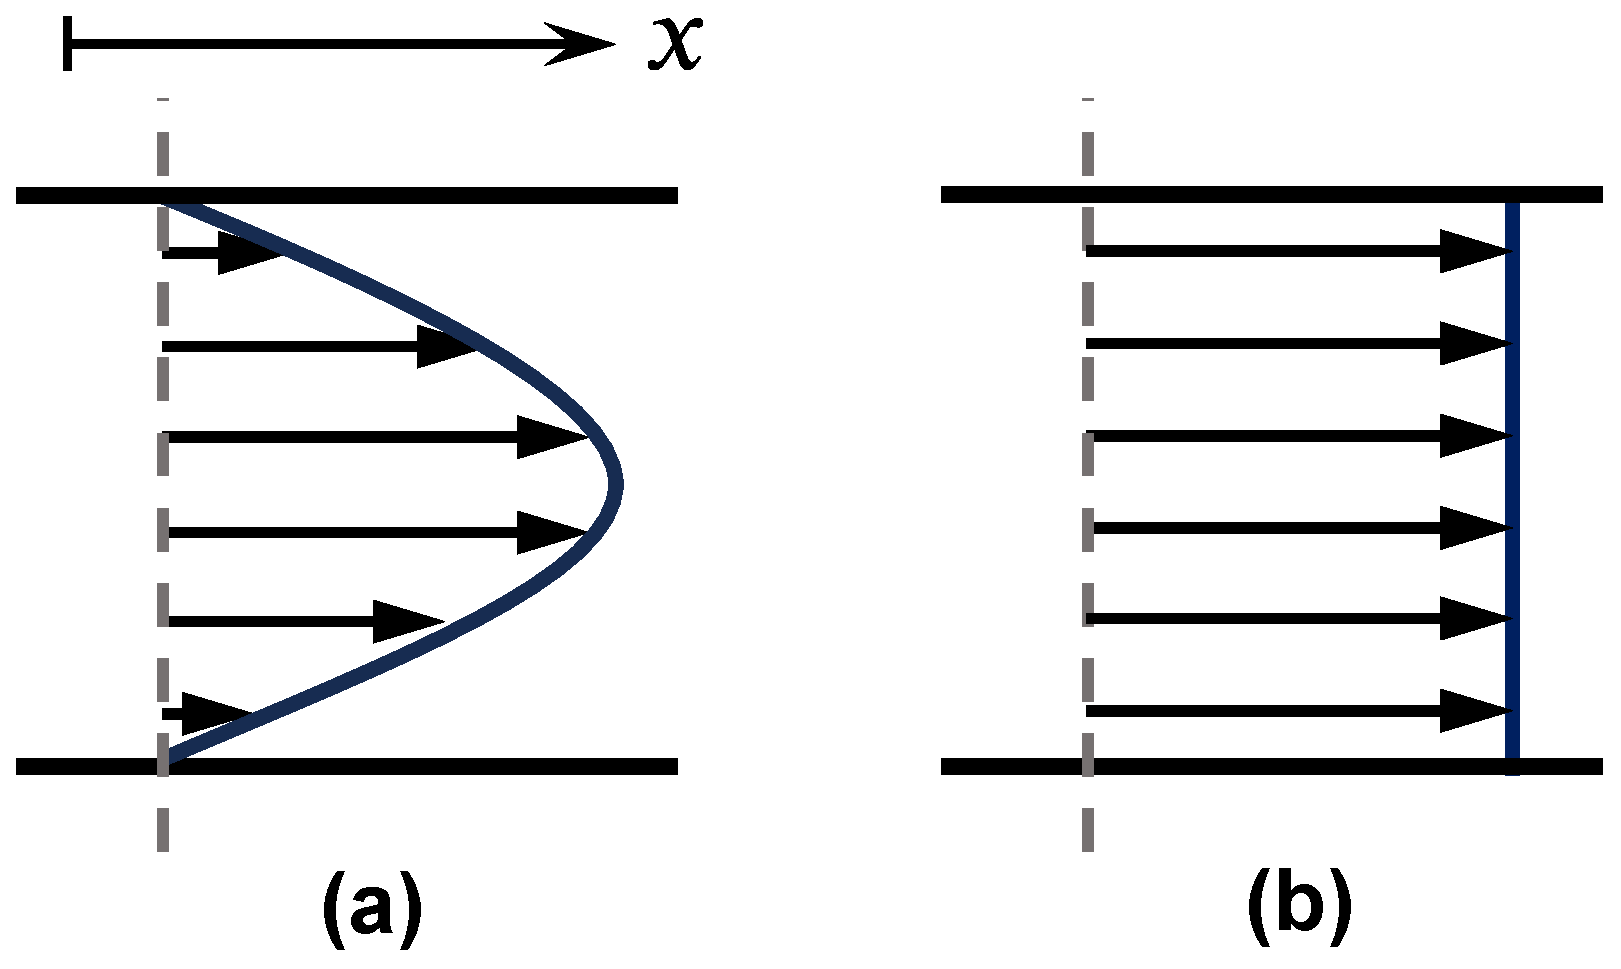
\includegraphics[width=.3\textwidth]{img/viscid_inviscid_profs.eps}
    \caption {The velocity profile of flow between two parallel plates when the fluid is (a) affected by viscosity, (b) inviscid.}
\end{figure}

\vfill
{\small \color{gray}Drafted by B. Li, H. El Nashar, and C. H. Yap,  \today}
% \thispagestyle{empty}
\newgeometry{margin=1.8cm}
\mbox{}
\vfill    
\begin{figure}[H]
    \includegraphics[right]{images/by-nc.eps}
\end{figure}
\textit{This work is licensed under a Creative Commons Attribution-NonCommercial 4.0 International License.}


\end{document}

